\documentclass[12pt]{article}

\usepackage{amsmath, mathtools}
\usepackage{amsfonts}
\usepackage{amssymb}
\usepackage{graphicx}
\usepackage{colortbl}
\usepackage{xr}
\usepackage{hyperref}
\usepackage{longtable}
\usepackage{xfrac}
\usepackage{tabularx}
\usepackage{float}
\usepackage{siunitx}
\usepackage{booktabs}
\usepackage{caption}
\usepackage{pdflscape}
\usepackage{afterpage}   
\usepackage{graphicx}

\usepackage[round]{natbib}

%\usepackage{refcheck}

\hypersetup{
	bookmarks=true,         % show bookmarks bar?
	colorlinks=true,       % false: boxed links; true: colored links
	linkcolor=red,          % color of internal links (change box color with
	%linkbordercolor)
	citecolor=green,        % color of links to bibliography
	filecolor=magenta,      % color of file links
	urlcolor=cyan           % color of external links
}

%% Comments

\usepackage{color}

\newif\ifcomments\commentstrue %displays comments
%\newif\ifcomments\commentsfalse %so that comments do not display

\ifcomments
\newcommand{\authornote}[3]{\textcolor{#1}{[#3 ---#2]}}
\newcommand{\todo}[1]{\textcolor{red}{[TODO: #1]}}
\else
\newcommand{\authornote}[3]{}
\newcommand{\todo}[1]{}
\fi

\newcommand{\wss}[1]{\authornote{blue}{SS}{#1}} 
\newcommand{\plt}[1]{\authornote{magenta}{TPLT}{#1}} %For explanation of the template
\newcommand{\an}[1]{\authornote{cyan}{Author}{#1}}


\newcommand{\progname}{Software Eng 4G06} % PUT YOUR PROGRAM NAME HERE
\newcommand{\authname}{Team 2, Parnas' Pals
	\\ Jared Bentvelsen
	\\ Bassel Rezkalla
	\\ Yuvraj Randhawa
	\\ Dimitri Tsampiras
	\\ Matthew McCracken} % AUTHOR NAMES                  

\usepackage{hyperref}
\hypersetup{colorlinks=true, linkcolor=blue, citecolor=blue, filecolor=blue,
	urlcolor=blue, unicode=false}
\urlstyle{same}



% For easy change of table widths
\newcommand{\colZwidth}{1.0\textwidth}
\newcommand{\colAwidth}{0.13\textwidth}
\newcommand{\colBwidth}{0.82\textwidth}
\newcommand{\colCwidth}{0.1\textwidth}
\newcommand{\colDwidth}{0.05\textwidth}
\newcommand{\colEwidth}{0.8\textwidth}
\newcommand{\colFwidth}{0.17\textwidth}
\newcommand{\colGwidth}{0.5\textwidth}
\newcommand{\colHwidth}{0.28\textwidth}

% Used so that cross-references have a meaningful prefix
\newcounter{defnum} %Definition Number
\newcommand{\dthedefnum}{GD\thedefnum}
\newcommand{\dref}[1]{GD\ref{#1}}
\newcounter{datadefnum} %Datadefinition Number
\newcommand{\ddthedatadefnum}{DD\thedatadefnum}
\newcommand{\ddref}[1]{DD\ref{#1}}
\newcounter{theorynum} %Theory Number
\newcommand{\tthetheorynum}{T\thetheorynum}
\newcommand{\tref}[1]{T\ref{#1}}
\newcounter{tablenum} %Table Number
\newcommand{\tbthetablenum}{T\thetablenum}
\newcommand{\tbref}[1]{TB\ref{#1}}
\newcounter{assumpnum} %Assumption Number
\newcommand{\atheassumpnum}{P\theassumpnum}
\newcommand{\aref}[1]{A\ref{#1}}
\newcounter{goalnum} %Goal Number
\newcommand{\gthegoalnum}{P\thegoalnum}
\newcommand{\gsref}[1]{GS\ref{#1}}
\newcounter{instnum} %Instance Number
\newcommand{\itheinstnum}{IM\theinstnum}
\newcommand{\iref}[1]{IM\ref{#1}}
\newcounter{reqnum} %Requirement Number
\newcommand{\rthereqnum}{P\thereqnum}
\newcommand{\rref}[1]{R\ref{#1}}
\newcounter{nfrnum} %NFR Number
\newcommand{\rthenfrnum}{NFR\thenfrnum}
\newcommand{\nfrref}[1]{NFR\ref{#1}}
\newcounter{lcnum} %Likely change number
\newcommand{\lthelcnum}{LC\thelcnum}
\newcommand{\lcref}[1]{LC\ref{#1}}

\usepackage{fullpage}

\newcommand{\deftheory}[9][Not Applicable]
{
	\newpage
	\noindent \rule{\textwidth}{0.5mm}
	
	\paragraph{RefName: } \textbf{#2} \phantomsection 
	\label{#2}
	
	\paragraph{Label:} #3
	
	\noindent \rule{\textwidth}{0.5mm}
	
	\paragraph{Equation:}
	
	#4
	
	\paragraph{Description:}
	
	#5
	
	\paragraph{Notes:}
	
	#6
	
	\paragraph{Source:}
	
	#7
	
	\paragraph{Ref.\ By:}
	
	#8
	
	\paragraph{Preconditions for \hyperref[#2]{#2}:}
	\label{#2_precond}
	
	#9
	
	\paragraph{Derivation for \hyperref[#2]{#2}:}
	\label{#2_deriv}
	
	#1
	
	\noindent \rule{\textwidth}{0.5mm}
	
}

\begin{document}

\title{Software Requirements Specification for \progname: subtitle describing software} 
\author{\authname}
\date{\today}
	
\maketitle

~\newpage

\pagenumbering{roman}

\tableofcontents

~\newpage

\section*{Revision History}

\begin{tabularx}{\textwidth}{p{3cm}p{2cm}X}
\toprule {\bf Date} & {\bf Version} & {\bf Notes}\\
\midrule
October 1, 2022 & 1.0 & Volere template outline, Functional Requirements\\
October 5, 2022 & 1.1 & Completed and submitted SRS document\\
\bottomrule
\end{tabularx}

~\newpage

\section{Project Drivers}
\subsection{The Purpose of the Project}
  \subsubsection{The User Business or Background of the Project Effort}
  \noindent
  With the increase in media consumption across the world, there has been a greater focus on several previously underrepresented or inaccessable niches, such as health and fitness. Despite the growth and presence of fitness in social media, there are still large barriers to entry that make it intimidating to get started or get accurate information that would aid individuals in their fitness journeys. A lot of the media available online is either behind a paywall, or structured in undigestible video and written formats. The lack of a free, centralized system that contains media generated and verified by fitness enthusiasts alike spurred the idea for this application. This application aims to bridge the gap that exists in the online fitness world by allowing individuals to create and track workouts of their own, search and share workouts created by others, and review and discuss what they find personally works and doesn't work for them. Creating a collaborative online fitness environment allows individuals to start or expand their fitness journey without looking in numerous locations or paying money for programs that may not work for them. 
\subsection{Stakeholders}
\begin{enumerate}
	\item Fitness Enthusiasts - Anyone interested in exploring other fitness routines, creating their own routines, and tracking their own personal progression towards goals.
	\item Personal Trainers - Olympian provides the ideal platform for trainers to share routines and goals with their clients.
	\item Fitness Advertisers - One avenue of monetization that Olympian could take is running advertisements. Although these advertisements could fall into any category, the largest stakeholders will be Fitness Advertisers,
	as the users of Olympian will be heavily involved with fitness, and thus most likely to buy fitness products.
\end{enumerate} 

\section{Project Constraints}
\subsection{Mandated Constraints} 
\subsubsection{Solution Constraints}
\begin{enumerate}
	\item
	\textbf{Description: } The product shall operate its back-end server with Node.js. \\
	\textbf{Rationale: } The product depends on the functionality provided by many libraries unique to Node.js. \\
	\textbf{Fit Criterion: } All back-end server libraries used are Node.js libraries, with a Node.js back-end. \\
\end{enumerate}
\subsubsection{Implementation Environment of the Current System}
The product will be launched as a web-app on the internet, and as a mobile app. There is no hardware or otherwise physical integration of the product.
\subsubsection{Partner or Collaborative Applications}
N/A
\subsubsection{Off-the-Shelf Software}
N/A
\subsubsection{Anticipated Workplace Environment}
N/A
\subsubsection{Schedule Constraints}
The product timeline will follow the schedule as laid out in the course outline by Dr. Smith. \\
\newline
\begin{tabular}{ p{9.7cm} l r}
	
	Team Formed, Project Selected & September 19 & 0\% \\
	
	Problem Statement, Development Plan & September 26 &
	2\% \\
	
	Requirements Document Revision 0 & October 5 & 5$\%^{\dagger, \ddagger}$ \\
	
	Hazard Analysis 0 & October 19 & 3$\%^\dagger$ \\
	
	V\&V Plan Revision 0 & November 2 & 5$\%^{\dagger, \ddagger}$ \\
	
	Proof of Concept Demonstration & November 14--25 & 5$\%^*$ \\
	
	Design Document Revision 0 & January 18 & 5$\%^{\dagger, \ddagger}$ \\
	
	Revision 0 Demonstration & February 6--February 17 & 10$\%^*$\\
	
	V\&V Report Revision 0 & March 8 & 5$\%^{\dagger, \ddagger}$ \\
	
	Final Demonstration (Revision 1) & March 20--March 31 &  20$\%^*$ \\
	
	EXPO Demonstration & April TBD & 10$\%^*$ \\
	
	Final Documentation (Revision 1)\newline 
	- Problem Statement\newline
	- Development Plan\newline
	- Requirements Document\newline
	- Hazard Analysis\newline
	- Design Document\newline
	- V\&V Plan\newline
	- V\&V Report\newline
	- User's Guide\newline
	- Source Code\newline &  April 5 & 30$\%^{*, \ddagger}$\\
	
\end{tabular}
\subsubsection{Budget Constraints}
N/A
\subsubsection{Enterprise Constraints}
N/A

\subsection{Naming Conventions and Terminology}
Below is a glossary of terms, acronyms and abbreviations used by stakeholders involved in the product's scope:
\begin{itemize}
	\item \textbf{Repetitions: } The number of times a motion will be repeated.
	\item \textbf{Exercise: } An entity describing a physical movement to be performed with optional descriptors and any combination of the following quantifiers: Repetitions, Sets, Weight, Distance, Time, and Rest Time. 
	\item \textbf{Routine: } A routine (or workout routine) is composed of a sequence of exercises performed in order.
\end{itemize}
\subsection{Relevant Facts and Assumptions}
N/A
\section{Functional Requirements}
\subsection{The Scope of the Work}
\subsubsection{The Current Situation}
N/A
\subsubsection{The Context of the Work}
N/A
\subsubsection{Work Partitioning}
\begin{center}
\begin{tabular}{ |p{5cm}|p{5cm}|p{5cm}| } 
 \hline
 \textbf{Event Name} & \textbf{Input and Output} & \textbf{Summary} \\ 
 Creating a Program  & Program Creation \(input\) & Finalizing all program creation inputs from user  \\ 
 Leaving a review on a user's post & Writing a review \(input\) & Commenting and proving a numeric value for program value \\
 Searching for a Program & Program Search \(input\) & Searching and browsing for a specific program or type of program based on search parameters  \\ 
 Sorting search results & Results sorted and displayed \(output\) & Sorting search results in a relevant way that is useful to the user \\ 
 Adding performed sets and reps for exercise & Entering rep and set information \(input\) & Tracking workout information by adding sets and reps performed during exercise \\ 
 Registering an account & Creating a new account \(input\) & This creates a new user and appends it to the database \\ 
 Adding program to profile  & Appending a program to personal profile \(input\) & Users can add programs they find to their profiles to use a later time or immediately \\ 
 Logging into account & Entering account information \(input\) & This authenticates and authorizes the user to access their account  \\ 
 Providing users with suggested programs and workouts & Generating and displaying programs and workouts tailored to individual users \(output\) & Using specific algorithms that find programs that suit the users needs \\ 
 Providing user with statistics & Generating and displaying statistics \(output\) & This will show users statistics they wouldn't otherwise know about. \\ 
 \hline
\end{tabular}
\end{center}
\subsection{Business Data Model and Data Directory}
N/A
\subsection{The Scope of the Product}
\subsubsection{Product Boundary}
N/A
\subsubsection{Use cases}

\begin{itemize}
	\item View posted workout routine 
	\begin{enumerate}
		\item View other user's fitness progress
		\item Add Personal Workout List
		\item View workout Author
		\item Review workout
	\end{enumerate}
	
	\item Browse Workout routines
	\begin{enumerate}
		\item Filter routines
	\end{enumerate}
	
	\item View Another User's Profile
	\begin{enumerate}
		\item View user's created routines
	\end{enumerate}
	
	\item Create User Profile
	\begin{enumerate}
		\item Setup profile description
		\item Setup attributes
	\end{enumerate}
	
	\item Edit User Profile
	
	\item Start workout routine
	\begin{enumerate}
		\item Track exercises in-progress
		\item Track personal Quantifiers
		\item Update current routine
	\end{enumerate}
	
	
	\item Create workout routine
	\begin{enumerate}
		\item Post workout routine
		\item Categorize routine
		\item Add workout length details
		\item Add exercise 
		\begin{enumerate}
			\item Add Quantifier
			\item Add Workout Descriptions
		\end{enumerate}
	\end{enumerate}
	
	\item Edit Routine
	\item Remove Routine
	\item View Workout List
\end{itemize}

\subsubsection{Use case Diagram}
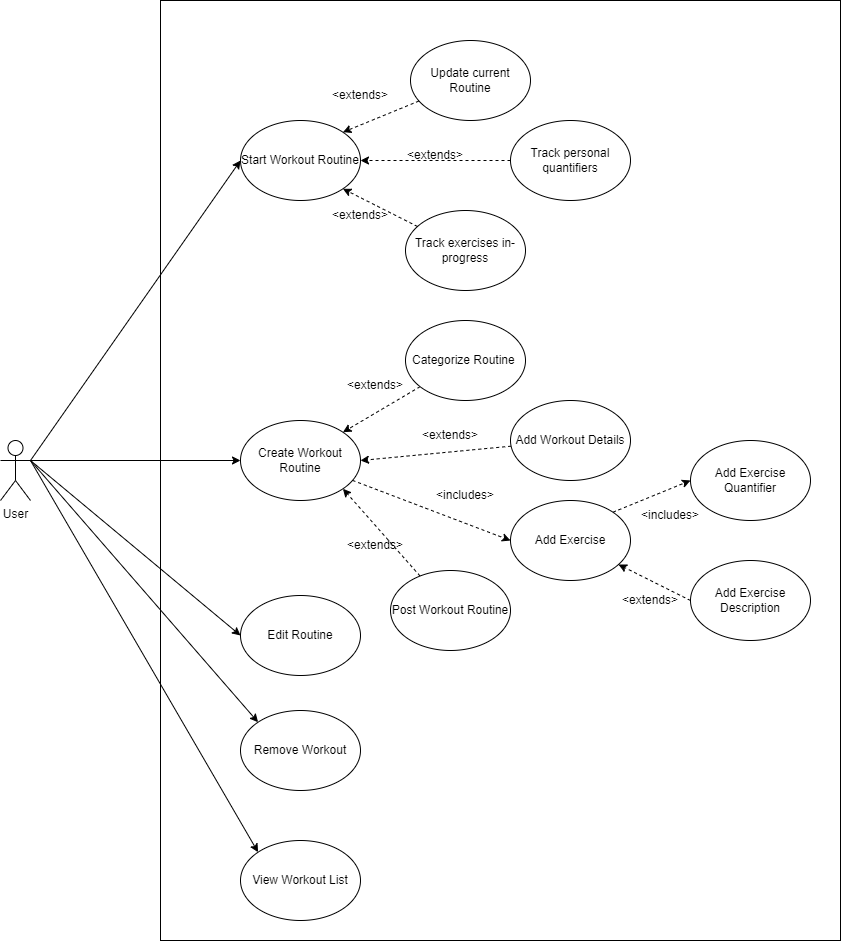
\includegraphics[scale=0.5]{srs_usecase_diagram_routines}
\newpage
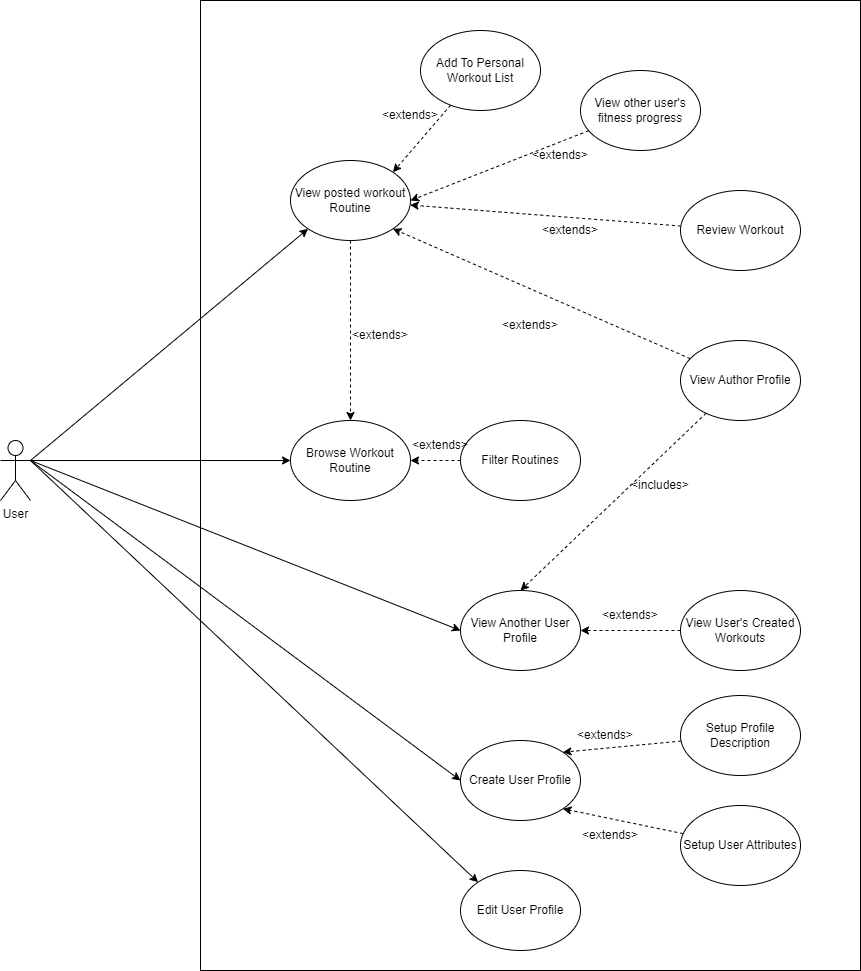
\includegraphics[scale=0.5]{srs_usecase_diagram_profiles}

\subsection{Functional Requirements}
\noindent \begin{itemize}

\item[R\refstepcounter{reqnum}\thereqnum \label{R_Inputs}:]
Description: The system shall allow the user to create a workout routine.
\\ Rationale: To allow the user to save their own workout routines.
\\ Fit Criterion: The user created routines are accessible after creation.

\item[R\refstepcounter{reqnum}\thereqnum \label{R_Inputs}:]
Description: The system shall allow the user to add and remove individual exercises in order to a created workout routine, with a maximum of 20 exercises per workout routine.
\\ Rationale: A workout routine is composed of a sequence of exercises performed in order, which the user should be able to add and remove as they wish to create the desired routine.
\\ Fit Criterion: The user is able to add and remove exercises from a created workout routine.

\item[R\refstepcounter{reqnum}\thereqnum \label{R_Inputs}:]
Description: The system shall allow the user to add or remove quantifiers to a given exercise.
\\ Rationale: A single exercise requires quantifiers including but not limited to sets, reps, weight (light, medium, heavy), time, rest time to adequately specify how it is to be performed within a given routine.
\\ Fit Criterion: The user is able to add quantifiers to a given exercise.

\item[R\refstepcounter{reqnum}\thereqnum \label{R_Inputs}:]
Description: The system shall allow the user to publicly post a workout routine.
\\ Rationale: To be able to display their workout routine to other users.
\\ Fit Criterion: On publication of a routine, another user should be able to access and view the routine.


\item[R\refstepcounter{reqnum}\thereqnum \label{R_Inputs}:]
Description: The system shall allow a user to save and view a performed workout.
\\ Rationale: To allow a user to keep track of their current workout, and review their previous workouts when doing them again.
This is especially helpful for ensuring progressive overload. That is, doing a little bit more than last time.
\\ Fit Criterion: The user is able to save a performed workout and review that data in the future.

\item[R\refstepcounter{reqnum}\thereqnum \label{R_Inputs}:]
Description: The product shall allow a user to browse and search for workout routines.
\\ Rationale: To make publicly posted workout routines discoverable and for users to find routines that cater their fitness goals.
\\ Fit Criterion: The user is able to browse and search for workout routines. The returned routines contain words that the user searched for.

\item[R\refstepcounter{reqnum}\thereqnum \label{R_Inputs}:]
Description: The system should allow a user to create a profile, with a username between 1 and 25 characters.
\\ Rationale: To display social, informational content to other users.
\\ Fit Criterion: The user is able to create a profile.


\item[R\refstepcounter{reqnum}\thereqnum \label{R_Inputs}:]
Description: The system shall allow a user to search for and view another user's profile.
\\ Rationale: To allow a user to determine if another user has similar fitness goals or similar workout routines.
\\ Fit Criterion: The user is able to view the profile of another user after searching for the target profile username.

\item[R\refstepcounter{reqnum}\thereqnum \label{R_Inputs}:]
Description: The system shall allow the user to create and view a goal in the form of an exercise and a metric pair. For example, ``Bench press - 100kg".
\\ Rationale: This allows the user to set and witness progression towards their fitness goals.
\\ Fit Criterion: The user is able to create and view goals.

\item[R\refstepcounter{reqnum}\thereqnum \label{R_Inputs}:]
Description: The system shall allow the user to create progress points towards a specific goal.
A progress point must be associated with a one specific goal, and must exist as a date metric pair. For example, ``09/04/22 - 96kg" under a ``Bench Press - 100kg" goal. The metric type must match the goal metric type, for example kg.
\\ Rationale: Being able to track progress towards set goals can help encourage more progression until the goal is reached.
\\ Fit Criterion: The user is able to create progress points towards specific goals.

\item[R\refstepcounter{reqnum}\thereqnum \label{R_Inputs}:]
Description: The product shall be able to visually display fitness progress towards set fitness goals.
\\ Rationale: To help the user determine progress towards fitness goals.
\\ Fit Criterion: The user is able to view progress points toward a set fitness goal.


\end{itemize}

%\plt{Every IM should map to at least one requirement, but not every requirement
%  has to map to a corresponding IM.}

\section{Nonfunctional Requirements}

%\plt{List your nonfunctional requirements.  You may consider using a fit
%  criterion to make them verifiable.}
%\plt{The goal is for the nonfunctional requirements to be unambiguous, abstract
%  and verifiable.  This isn't easy to show succinctly, so a good strategy may be
%to give a ``high level'' view of the requirement, but allow for the details to
%be covered in the Verification and Validation document.}
%\plt{An absolute requirement on a quality of the system is rarely needed.  For
%  instance, an accuracy of 0.0101 \% is likely fine, even if the requirement is
%  for 0.01 \% accuracy.  Therefore, the emphasis will often be more on
%  describing now well the quality is achieved, through experimentation, and
%  possibly theory, rather than meeting some bar that was defined a priori.}
%\plt{You do not need an entry for correctness in your NFRs.  The purpose of the
%  SRS is to record the requirements that need to be satisfied for correctness.
%  Any statement of correctness would just be redundant. Rather than discuss
%  correctness, you can characterize how far away from the correct (true)
%  solution you are allowed to be.  This is discussed under accuracy.}
\subsection{Look and Feel Requirements}
\subsubsection{Appearance Requirements}
\noindent \begin{itemize}
	\item N/A
\end{itemize}
\subsubsection{Style Requirements}
\noindent \begin{itemize}
	\item[NFR\refstepcounter{nfrnum}\thenfrnum:]
	The product shall be appear minimal and straightforward.
\end{itemize}
\subsection{Usability and Humanity Requirements}
\subsubsection{Ease of Use Requirements}
\noindent \begin{itemize}
	\item[NFR\refstepcounter{nfrnum}\thenfrnum:]
	The product shall use fonts of readable size to the target user group.
\end{itemize}
\subsubsection{Personalization and Internationalization Requirements}
\noindent \begin{itemize}
	\item[NFR\refstepcounter{nfrnum}\thenfrnum:]
	The product shall allow the user to select a chosen language.
\end{itemize}
\subsubsection{Learning Requirements}
\noindent \begin{itemize}
	\item[NFR\refstepcounter{nfrnum}\thenfrnum:]
	The product shall be able to be used by untrained fitness enthusiasts and amateurs alike, who receive no training before using it.
\end{itemize}
\subsubsection{Understandability and Politeness Requirements}
\noindent \begin{itemize}
	\item[NFR\refstepcounter{nfrnum}\thenfrnum:]
	The product shall use symbols and pictures to provide users with an intuitive and efficient experience.
\end{itemize}
\subsubsection{Accessibility Requirements}
\noindent \begin{itemize}
	\item[NFR\refstepcounter{nfrnum}\thenfrnum:]
	The product shall be usable by users with hearing loss or partial blindness.
\end{itemize}
\noindent \begin{itemize}
	\item[NFR\refstepcounter{nfrnum}\thenfrnum:]
	The product shall make use of sufficiently contrasting colours.
\end{itemize}
\subsection{Performance Requirements}
  \subsubsection{Speed and Latency Requirements}
    \noindent\begin{itemize}
      \item[NFR\refstepcounter{nfrnum}\thenfrnum:] 
        Users shall be able to input or update a program within 10 seconds.
    \end{itemize}
  \subsubsection{Safety-Critical Requirements}
    \noindent\begin{itemize}
      \item NA
    \end{itemize}
  \subsubsection{Precision or Accuracy Requirements}
    \noindent\begin{itemize}
      \item[NFR\refstepcounter{nfrnum}\thenfrnum:] 
        The average of the ratings per post shall be accurate to 2 decimal places.
    \end{itemize}
  \subsubsection{Reliability and Availability Requirements}
    \noindent\begin{itemize}
      \item[NFR\refstepcounter{nfrnum}\thenfrnum:] 
        The application shall achieve a 95 percent uptime.
    \end{itemize}
  \subsubsection{Robustness or Fault-Tolerance Requirements}
    \noindent\begin{itemize}
		\item N/A
    \end{itemize}
  \subsubsection{Capacity Requirements}
    \noindent\begin{itemize}
      \item[NFR\refstepcounter{nfrnum}\thenfrnum:] 
        The application shall support 100 simultaneous users per hour. 
    \end{itemize}
  \subsubsection{Scalability or Extensibility Requirements}
    \noindent\begin{itemize}
      \item[NFR\refstepcounter{nfrnum}\thenfrnum:] 
        The application should be able to support 1000 users per hour within a year of its creation.
    \end{itemize}
  \subsubsection{Longevity Requirements}
    \noindent\begin{itemize}
		\item N/A
    \end{itemize}

\subsection{Operational and Environmental Requirements}
  \subsubsection{Expected Physical Environment}
    \noindent\begin{itemize}
		\item N/A
    \end{itemize}
  \subsubsection{Requirements for Interfacing with Adjacent Systems}
    \noindent\begin{itemize}
      \item[NFR\refstepcounter{nfrnum}\thenfrnum:] 
        The application shall operate on iOS devices and Android devices.
    \end{itemize}  
  \subsubsection{Productization Requirements}
    \noindent\begin{itemize}
		\item N/A
    \end{itemize} 
  \subsubsection{Release Requirements}
    \noindent\begin{itemize}
		\item N/A
    \end{itemize}  

\subsection{Maintainability and Support Requirements}
  \subsubsection{Maintenance Requirements}
    \noindent \begin{itemize}
      \item[NFR\refstepcounter{nfrnum}\thenfrnum:]
        The application must inform users when maintenance is taking place and must warn them at least 1 day in advance. 
    \end{itemize}
  \subsubsection{Supportability Requirements}
    \noindent \begin{itemize}
      \item N/A
    \end{itemize}
  \subsubsection{Adaptability Requirements}
    \noindent \begin{itemize}
		\item N/A
    \end{itemize}

\subsection{Security Requirements}
  \subsubsection{Access Requirements}
    \noindent \begin{itemize}
      \item[NFR\refstepcounter{nfrnum}\thenfrnum:]
        The application must not display other users private details to the user.
    \end{itemize}
  \subsubsection{Integrity Requirements}
    \noindent \begin{itemize}
      \item[NFR\refstepcounter{nfrnum}\thenfrnum:]
       Passwords must be encrypted with SHA-256 when stored.
    \end{itemize}

  \subsubsection{Privacy Requirements}
    \noindent \begin{itemize}
      \item[NFR\refstepcounter{nfrnum}\thenfrnum:]
        The application must use OAuth protocols to verify communication between the client and server.
    \end{itemize}

  \subsubsection{Audit Requirements}
    \noindent \begin{itemize}
      \item[NFR\refstepcounter{nfrnum}\thenfrnum:]
        Data will be stored in a secure database. When data is deleted or edited a record of this data will be kept for up to 30 days.
    \end{itemize}
  \subsubsection{Immunity Requirements}
    \noindent \begin{itemize}
      \item N/A
    \end{itemize}



\subsection{Cultural Requirements}
  \subsubsection{Cultural Market Requirements}
    \noindent \begin{itemize}
      \item[NFR\refstepcounter{nfrnum}\thenfrnum:]
        The application will filter out profanities and flag repeat offenders for suspension.
      \item[NFR\refstepcounter{nfrnum}\thenfrnum:]
        The application will allow users to report offensive content and remove it from their feed.
    \end{itemize}
  \subsubsection{Cultural Diversity and Inclusion Requirements}
    \noindent \begin{itemize}
      \item[NFR\refstepcounter{nfrnum}\thenfrnum:]
        Users can optionally specify their gender, age, and race. Gender and age will be used to cater the content for individuals feeds.
    \end{itemize}

\subsection{Legal Requirements}
  \subsubsection{Legal Compliance Requirements}
    \noindent \begin{itemize}
      \item[NFR\refstepcounter{nfrnum}\thenfrnum:]
        The use of data will comply with the Data Protection Act.
    \end{itemize}
  \subsubsection{Standards Compliance Requirements}
    \noindent \begin{itemize}
      \item N/A
    \end{itemize}
	\section{Traceability Matrices and Graphs}
	
	\begin{table}[h!]
		\centering
		\begin{tabular}{|c|c|c|c|c|c|c|c|c|c|c|c|}
			\hline
			& R1 & R2 & R3 & R4 & R5 & R6 & R7 & R8 & R9 & R10 & R11 \\ \hline
			NFR4 &X & & & & & & & & & & \\ \hline
			NFR8 &X &X &X & & & & & & & & \\ \hline
			NFR9 & & & & & & &X & & & & \\ \hline % 6
			NFR10 & & & & & & &X &X & & & \\ \hline % 7,8
			NFR11 & & & & & & &X &X & & &\\ \hline % 7,8
			NFR12 & & & & & & &X &X & & & \\ \hline % 7,8
			NFR13 &X & & & & &X &X & & & & \\ \hline % 1,7,8
			NFR18 &X & & & &X & &X & &X &X &X \\ \hline % 11,10,9,7,5,1
			NFR20 & & & & & &X & &X & & & \\ \hline % 6,8
			NFR22 &X & & & &X & &X & &X &X &X \\ \hline % 11,10,9,7,5,1	
		\end{tabular}
		\caption{NonFunctional to Functional Requirement Dependency Matrix}
		\label{Table:R_trace}
	\end{table}

	\newpage
	
	\section{Project Issues}
		\subsection{Open Issues}
			\begin{itemize}
				\item \textbf{Issue 1:} Users may have discomfort using an app to track their workouts over the traditional pen and paper method. The business event of tracking personal quantifiers is of concern with this issue.
				
				\item \textbf{Issue 2:} It may be unfavourable to users with existing programs and workout data to migrate to a new application.
				
				\item \textbf{Issue 3:} Users' personal methods of working out - various quirks and features - may not be covered by the app's program creation capabilities.
				
				\item \textbf{Issue 4:} There is a concern with the app’s compatibility with various devices. Integral UI/UX features of the app such has haptics, pop-ups, and dragging features may not work with various devices - hindering the overall experience for some users.
				
			\end{itemize}
		
		\subsection{Off the Shelf Solutions}
			\subsubsection{Ready Made Products}
		
				\noindent TeamBuildr
				\begin{itemize}
				\item TeamBuildr is an exercise programming app for large groups used at a professional level. Used for teams, specifically at a high level. There is no present social aspect. It is also a paid service.
				\item Program creation is a very complex process. This app has a solution that has been tried and tested by multiple users at a high level. 
				\end{itemize}
				
				\noindent JEFIT
				\begin{itemize}
				\item JEFIT lets you create and track workouts. It does not feature user-generated content but has paid template programs. It has functionality allowing users to post progress pictures. 
				\item JEFIT could be used as a foundation for adding required features if acquired.
				\end{itemize}
		
			\subsubsection{Reusable Components}
		
				\noindent One Rep Max Calculator
				\begin{itemize}
				\item The npm library one-rep-max, can be used to satisfy the requirements of providing user statistics. The library offers multiple recognized methods of calculating users' maximum weight for one repetition. 
				\item Event: Track Personal Quantifiers 
				\end{itemize}
				
				\noindent Content-Based Recommender 
				\begin{itemize}
				\item The npm library content-based-recommender can help display recommended content for the user based on user inputted parameters.
				\item This addresses the business event "filter routines". 
				\end{itemize}
		
			\subsubsection{Products that can be copied}
		
				\noindent Exercise Directory
				\begin{itemize}
				\item Exercise Directory provides a bulk directory of various exercises that can be directly copied as there is no legal ownership of an exercise.
				\end{itemize}
		
				\noindent HyperHuman API 
				\begin{itemize}
				\item HyperHuman API offers pre-built workout programs that can be used as basic templates. This is especially useful in the beginning stages of the app where user generated content is at a low. 
				\item This addresses the business event "browse programs". 
				\end{itemize}
		
		\subsection{New Problems}
			Not applicable.
		\subsection{Tasks}
			\begin{itemize}
			\item Determine which technologies will be used for the creation of this project (frontend framework, server language).
			\item  Design UX wire-frames for the application.
			\item  Design UI design mockups for the application.
			\item  Design UI components and testing for the application with front-end technology.
			\item  Create skeleton of API.
			\item  Revise requirement documents.
			\item  Implement test report.
			\end{itemize}
		\subsection{Migration to the New Product}
			The product will be deployed to the Apple App store first, then it will be added to the Google Play store once it has run without issue on the app store.
			This project is new, so no transition period is relevant.
		\subsection{Risks}
			\begin{itemize}
			\item User data breach. If users' data is leaked, there would be damaging ramifications on our reputation and our userbase.
			\item Failure of content moderation. Olympian is a social media application and as such is susceptible to being used for nefarious and hateful purposes. This is why content moderation will be vital in running this application.
			\end{itemize}
		\subsection{Costs}
			\begin{itemize}
			\item The cost of keeping a server that is always responsive to client requests. This has an estimated cost of \$25 per month.
			\item The cost of utilizing a database that can handle many reads and writes quickly. This has an estimated cost of \$10 per month.
			\item The cost of an Individual Developer Account needed to host all apps on the Apple App Store. This will cost USD\$99.
			\end{itemize}
		\subsection{User Documentation and Training}
			N/A
		\subsection{Waiting Room}
			\begin{itemize}
			\item The product must allow users to track their diet information and recommend diets based on calory intake.
			\item The product must algorithmically produce a "Recommended" feed filled with workouts selected for users based on their habits and interests.
			\item The product must include an optional networking feature where users can view the growth of similar users and track the steps taken to produce those improvements.
			\end{itemize}
		\subsection{Ideas for Solutions}
			The product should be built using React Native along with an Express.js backend and utilizing the Google Firestore suite for app management including database and storage. Pricing was collected with these services in mind and they fullfil the needs of the product.

	
	
	
	\section{Reference Material}
	
	This section records information for easy reference.
	
	
	\subsection{Abbreviations and Acronyms}
	
	\renewcommand{\arraystretch}{1.2}
	\begin{tabular}{l l} 
		\toprule		
		\textbf{symbol} & \textbf{description}\\
		\midrule 
		A & Assumption\\
		DD & Data Definition\\
		GD & General Definition\\
		GS & Goal Statement\\
		IM & Instance Model\\
		LC & Likely Change\\
		PS & Physical System Description\\
		R & Requirement\\
		SRS & Software Requirements Specification\\
		%\progname{} & \plt{put an expanded version of your program name here (as
		%	appropriate)}\\
		T & Theoretical Model\\
		\bottomrule
	\end{tabular}\\
	
	\newpage{}
	\section{Reflection Appendix}

	\subsection{Required Skills and Knowledge}
	\begin{itemize}
			
		\item Skill: \textbf{Team management}
		\\ Rationale: In order to organize deadlines, work distribution, project progression and team communication, having good team management principles will guide the team towards a positive and productive environment.
		\\ Team member: William Lee
		
		\item Skill: \textbf{Data \& Database management}
		\\ Rationale: Many components of this project will require data tracking and storage in a secure fashion.
		\\ Team member: William Lee
		
		\item Skill: \textbf{Mobile UI Development}
		\\ Rationale: As a mobile application, this product will need to have a fluid user interface.
		\\ Team member: Dimitri Tsampiras
		
		\item Skill: \textbf{Mobile Functionality Development}
		\\ Rationale: As a mobile application, this product will require knowledge in mobile development techniques and functions.
		\\ Team member: Matthew McCracken

		\item Skill: \textbf{Full Stack Development}
		\\ Rationale: As an application utilizing a client side, a server, and an online database, this product will require knowledge of how to integrate different layers of full stack applications.
		\\ Team member: Matthew McCracken
		
		\item Skill: \textbf{Software Communications}
		\\ Rationale: Data distribution and transferring will be required for communication between software layers. Having knowledge towards software communicaton will be required to have efficent communication.
		\\ Team member: Jared Bentvelsen
		
		\item Skill: \textbf{Document Organization and Writing}
		\\ Rationale: Having descriptive and effective writing will be required to increase usability and decrease the learning curve for users. Document organization will be instrumental to carrying out project principles and guiding the growth and development of the project.
		\\ Team member: Yuvraj Randhawa
		
		\item Skill: \textbf{Software Architecture and Structure}
		\\ Rationale: Having a sound software structure will increase development efficiency, simplicity and organization. With topic knowledge in this area, software management and testing will be made easy, saving time and effort for developers.
		\\ Team member: Bassel Rezkalla
		
		
	\end{itemize}
	\subsection{Approaches for Acquiring Skills and Knowledge}
	\begin{itemize}
		
		\item Skill: \textbf{Team management}
		\\ Approach 1: Attend group synergy meetings where we discuss goals for the project and weekly meetings to discuss issues.
		\\ Approach 2: Utilize Discord and GitLab's PR functionality to achieve organization and solid communication for all project deliverables.
		\\ Verdict: William will use Approach 1 to improve his Team Management ability. He has chosen this approach because it will bring him face to face with his team and align team goals.
		
		\item Skill: \textbf{Data \& Database management}
		\\ Approach 1: Make use of the many online tutorials, articles and existing solutions for database management to refer to and learn from.
		\\ Approach 2: Utilize notes, projects, and past tests from SFWRENG-3DB3, a class that all members of the group took, to achieve good database management practices.
		\\ Verdict: William will use Approach 2 to improve his database management skills. He has chosen this approach because he has a vast collection of documentation from SFWRENG-3DB3 and did well in the course.

		\item Skill: \textbf{Mobile UI Development}
		\\ Approach 1: Most mobile UI have well documented libraries to refer and learn from. Having design and prototyping sessions with the team before development will help improve good domain knowledge.
		\\ Approach 2: Figma is the resource we will use to mock up the frames of our application. It also has extensive documentation and tutorials we will complete.
		\\ Verdict: Dimitri will use Approach 2 to improve his Mobile UI Development skills. Figma is a valuable resource and familiarizing himself with it will improve his ability to provide quality mobile designs. By performing these tutorials, Dimitri will be exposed to other mobile designs to learn what works and what doesn't. 

		\item Skill: \textbf{Mobile Functionality Development}
		\\ Approach 1: We can explore the Touch API and its documentation to learn about the events emitted by the actions of mobile users.
		\\ Approach 2: Practice by converting existing applications to make them mobile responsive. Our group has experience making web applications but could practice mobile development by making these apps responsive.
		\\ Verdict: Matthew will use Approach 1 to improve his Mobile Functionality Development skills. He has chosen this strategy because the Touch API is essential for making mobile applications and he already has experience with responsive web development.
		
		\item Skill: \textbf{Full Stack Development}
		\\ Approach 1: Complete the Google Cloud Certified - Associate Cloud Engineer Certification. This will provide skills on deploying web applications and integrating Google Cloud Services.
		\\ Approach 2: Set up dummy clients and servers and practice hosting active client applications with simple UI.
		\\ Verdict: Matthew will use Approach 1 to improve his Full Stack Development skills. He has chosen this strategy because this certificate offers a more extensive and professional training than Matthew can achieve on his own. Additionally, Google's certificate will introduce him to many GCP services that the project will need to utilize.
		
		\item Skill: \textbf{Software Communications}
		\\ Approach 1: Perform Github beginner to intermediate tutorials.
		\\ Approach 2: Take a Coursera Course on Software Specification writing.
		\\ Verdict: Jared will use Approach 2 to improve his Software Communications skills. He has chosen this strategy because the Coursera course will show examples of correct specifications and teach him best practices which he can then pass on to the team.
		
		\item Skill: \textbf{Document Organization and Writing}
		\\ Approach 1: Practice writing in a journal to practice descriptive and clear writing.
		\\ Approach 2: Review notes from SFWRENG-3I03 to improve communication skills in an engineering context.
		\\ Verdict: Yuvraj will use Approach 2 to improve his Document Organization and Writing skills. He has chosen this strategy because this course provided lessons on writing in LaTeX and how to write clear software documents. 
		
		\item Skill: \textbf{Software Architecture and Structure}
		\\ Approach 1: Referring to common software structures and architectures will help create guidelines for making a catered solution for this product. Many university courses such as McMaster's SFWRENG-2AA4 and SFWRENG-3A04 discuss topics surrounding software architecture.
		\\ Approach 2: Hold group meeting to discuss common architecture styles and come to an agreement on how all developers will design this architecture. Synergy is important with multiple developers designing a core structure.
		\\ Verdict: Bassel will use Approach 2 to improve his Software Architecture and Structure skills. He has chosen this strategy because it is important for all developers to be on the same page regarding software architecture strategies.
	\end{itemize}
	
\end{document}
